\documentclass[logo,reportComp]{thesis}
\usepackage[cpp,pseudo]{mypackage}

\title{数字图像处理作业四}
\subtitle{}
\school{数据科学与计算机学院}
\author{陈鸿峥}
\classname{17大数据与人工智能}
\stunum{17341015}
\headercontext{数字图像处理作业}
\lstset{language=matlab}

\begin{document}

\maketitle

\section{彩色图像人脸检测}
基于颜色空间做人脸检测,即给定一张图片,将其中的人脸框出来。

\subsection{原理}
主要基于文献\cite{bib:face_recog}中总结的三种方法进行人脸检测,实际上都是在不同颜色空间中做阈值变换。

在不同颜色空间中的人脸检测需要满足以下条件:
\begin{itemize}
	\item RGB颜色空间:
	\[\begin{cases}
	R>95\land G>40\land B>20\land (\max\{R,G,B\}-\min\{R,G,B\})>15\\
	\quad\land |R-G|>15 \land R>G \land R>B & \text{均匀照明}\\
	R>20\land G>210\land B>170\land |R-G|<15 \land R>G \land R>B & \text{潜在照明}
	\end{cases}\]
	\item HSV颜色空间:
	\[V\geq 0.4\land 0.2\leq S\leq 0.8\land 0\leq H\leq 0.25\]
	\item YCbCr颜色空间:
	\[75<Cb<250\land 10<Cr<100\land Y>80\]
\end{itemize}

整体流程包括以下几步:
\begin{enumerate}
	\item 图像预处理
	\item 图像颜色空间的转换
	\item 基于阈值的图像分割
	\item 连通分量分析
	\item 标注出人脸并显示
\end{enumerate}

\subsection{实验结果与分析}
最终的人脸及图像标注如下面几幅图所示,可以看出在RGB空间及在YCrCb空间上做阈值切分还是能够比较好地将皮肤部分提取出来,但RGB空间会损失较多细节;而基于HSV空间的阈值分析尽管也能提取出皮肤,但仍有大部分皮肤未被提取出来。
同时我们也可以发现基于阈值的划分方法其实并没有办法很好地区分人脸和其他人体部分,因此基于阈值的划分方法只能做简单的人脸检测处理,并且其阈值也是需要经过精细调整才能达到比较好的效果。
\begin{figure}[H]
\centering
\begin{tabular}{c}
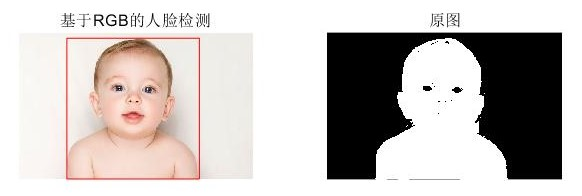
\includegraphics[width=0.8\linewidth]{fig/test01.jpg}\\
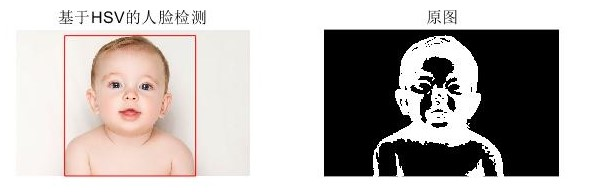
\includegraphics[width=0.8\linewidth]{fig/test02.jpg}\\
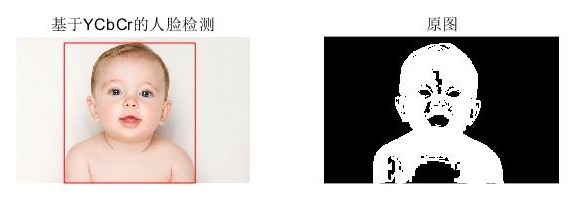
\includegraphics[width=0.8\linewidth]{fig/test03.jpg}
\end{tabular}
\end{figure}
\begin{figure}[H]
\centering
\begin{tabular}{c}
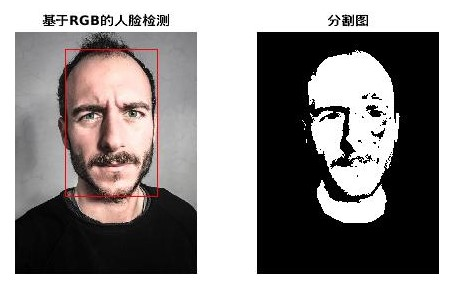
\includegraphics[width=0.8\linewidth]{fig/test11.jpg}\\
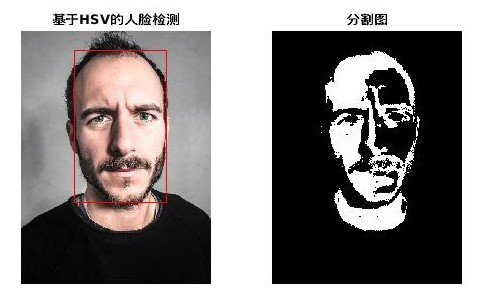
\includegraphics[width=0.8\linewidth]{fig/test12.jpg}\\
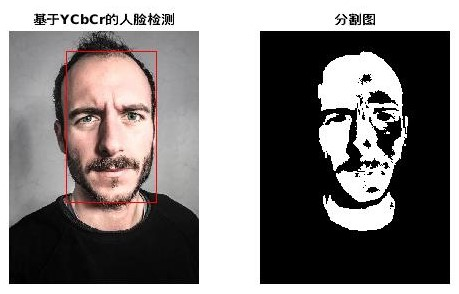
\includegraphics[width=0.8\linewidth]{fig/test13.jpg}
\end{tabular}
\end{figure}
\begin{figure}[H]
\centering
\begin{tabular}{c}
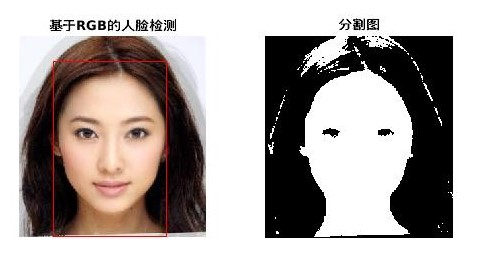
\includegraphics[width=0.8\linewidth]{fig/test21.jpg}\\
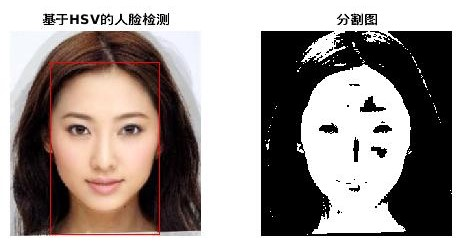
\includegraphics[width=0.8\linewidth]{fig/test22.jpg}\\
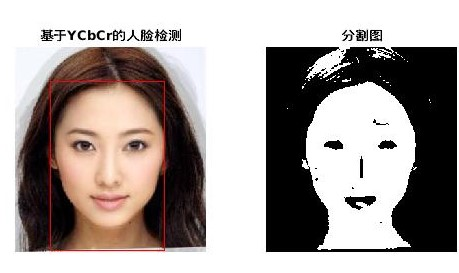
\includegraphics[width=0.8\linewidth]{fig/test23.jpg}
\end{tabular}
\end{figure}


\section{直方图均衡化}
观察对RGB图像的三个通道分别做直方图均衡,与对整个图像做直方图均衡是否一致。

\subsection{原理}
直方图均衡化在第一个Proj中已经完成,主要分为以下几个步骤:
\begin{itemize}
	\item 对原图片的像素进行统计,得到$[0,255]$中每一个灰度值的频数$n_k$,进而得到原图像的直方图
	\item 对原图像直方图进行归一化,由频数变为概率$p_r(r_k)=n_k/n$,实即概率质量函数(PMF)\footnote{注:由于是离散情况,故不是概率密度函数}
	\item 由概率质量函数求得累积质量函数(CMF)
	\[P(r_k)=\sum_{j=0}^kp_r(r_j)=\sum_{j=0}^k\frac{n_j}{n}\]
	\item 将原图像的灰度值作为$x$输入,从CMF中得到对应的输出值$y$,并且对$y$重新恢复尺度$[0,255]$,得到新图片中该位置的灰度值,即
	\[s_k=T(r_k)=255\cdot\sum_{j=0}^k\frac{n_j}{n}\]
	注意需要对$s_k$进行取整
	\item 对原图像中的每一个像素都这么操作,可以得到直方图归一化后的新图像
\end{itemize}
在这个实验中,则直接将其封装为一个函数,并分别对各通道和全图进行应用。

\subsection{实验结果与分析}
我主要采用了两幅图像进行直方图均衡化。
首先第一幅图是Lenna的人像,由于原本图像的对比度已经很清晰,因此经过全通道均衡化后的图片变化不大(但细看确实对比图提升了);而分通道均衡化后的图像则与原图会有巨大差异,主要体现在颜色上,如背景的浅红色经过分通道均衡化后被消除了。
\begin{figure}[H]
\centering
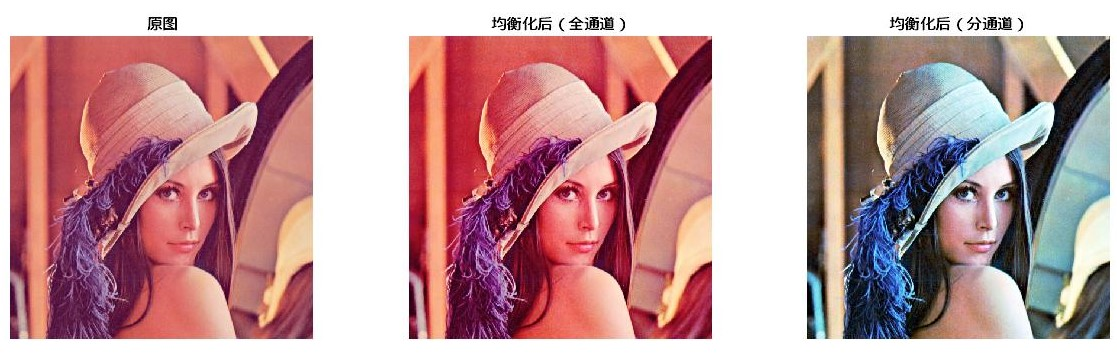
\includegraphics[width=\linewidth]{fig/histeq.jpg}
\end{figure}

第二幅图则是课本中比较暗的石头图片,这幅图片经过全通道直方图均衡化后,可以明显看出按部都被明显提升了;而分通道的均衡化同样也将对比度提升,同时图片不会偏蓝,会更加自然。
\begin{figure}[H]
\centering
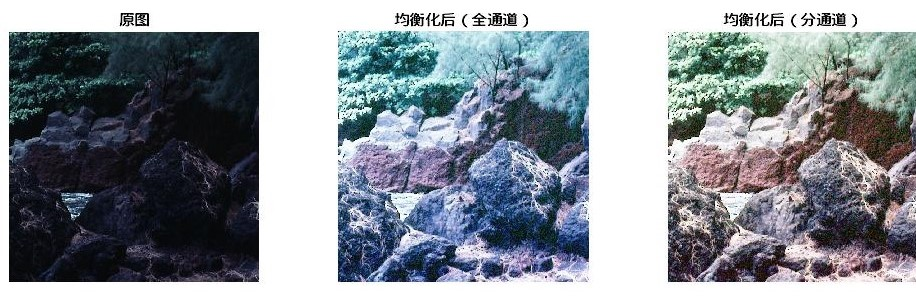
\includegraphics[width=\linewidth]{fig/histeq2.jpg}
\end{figure}

\section{带阻滤波器}
% Fig 5.5正弦噪声 Fig 5.16
利用带阻滤波器消除周期性噪声。

\subsection{原理}
仅仅阻断中间一圆环的频率分量,而其他分量均可正常通过。
下面是二维$n$阶巴特沃斯带阻滤波器的例子
\[H(u,v)=\frac{1}{1+\lrs{\frac{D(u,v)W}{D^2(u,v)-D_0^2}}^{2n}}\]
其中$D(u,v)$为距离中心点的距离,$D_0$为截止频率,$W$为带阻宽度。

\subsection{实验结果与分析}
原图被$\sin$的周期性噪声干扰。
通过调整圆环的位置及宽度,我们可以看到经过带阻滤波器后周期性噪声被有效消除了。
\begin{figure}[H]
\centering
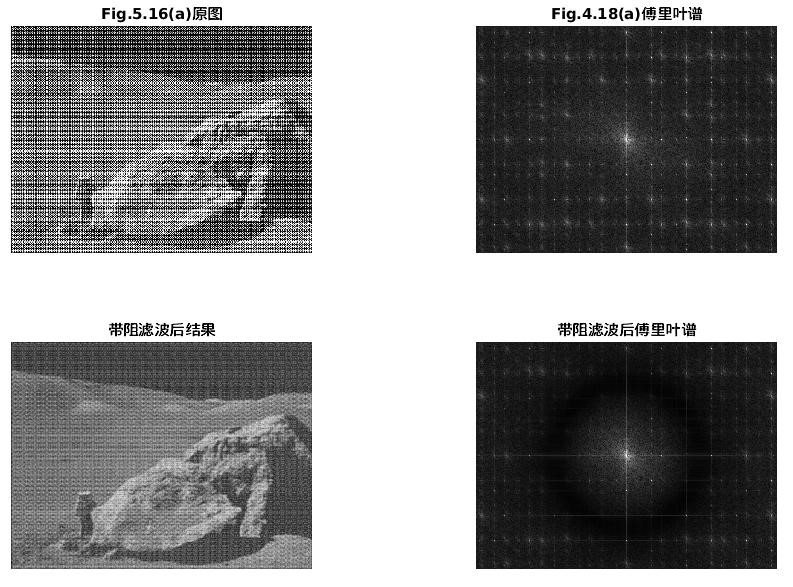
\includegraphics[width=\linewidth]{fig/br.jpg}
\end{figure}

\appendix\appendixconfig
\section{图像人脸检测代码}
\begin{lstlisting}
close all;clear all;clc;

I = imread('fig/TestImage.jpg');
I = imread('fig/test1.jfif');
I = imread('fig/test2.jpg');

BW_rgb = rgb_face(I);
BW_hsv = hsv_face(I);
BW_ycbcr = ycbcr_face(I);

bb_rgb = get_bb(BW_rgb);
bb_hsv = get_bb(BW_hsv);
bb_ycbcr = get_bb(BW_ycbcr);

figure, subplot(1,2,2);
imshow(BW_rgb)
title('`分割图'');
subplot(1,2,1);
imshow(I);
hold on;
rectangle('Position',bb_rgb,'EdgeColor','r');
title('`基于RGB的人脸检测'');

figure, subplot(1,2,2);
imshow(BW_hsv)
title('`分割图'');
subplot(1,2,1);
imshow(I);
hold on;
rectangle('Position',bb_hsv,'EdgeColor','r');
title('`基于HSV的人脸检测'');

figure, subplot(1,2,2);
imshow(BW_ycbcr)
title('`分割图'');
subplot(1,2,1);
imshow(I);
hold on;
rectangle('Position',bb_ycbcr,'EdgeColor','r');
title('`基于YCbCr的人脸检测'');

function bw = rgb_face(I)
	[m,n,c] = size(I);
	BW = zeros(m,n);
	for i = 1:size(I,1)
		for j = 1:size(I,2)
			R = I(i,j,1);
			G = I(i,j,2);
			B = I(i,j,3);
			v = [R,G,B];
			if (R > 95 && G > 40 && B > 20 && (max(v) - min(v)) > 15 && abs(R-G) > 15 && R > G && R > B) % day
			% if (R > 20 && G > 210 && B > 170 && abs(R-G) < 15 && R > G && R > B) % night
				BW(i,j) = 1;
			end
		end
	end
	bw = BW;
end

function bw = hsv_face(I)
	I_h = rgb2hsv(I);
	[m,n,c] = size(I_h);
	BW = zeros(m,n);
	for i = 1:m
		for j = 1:n
			h = I_h(i,j,1);
			s = I_h(i,j,2);
			v = I_h(i,j,3);
			if (v > 0.40 && s >= 0.2 && s <= 0.6 && h >= 0 && h <= 0.25)
				BW(i,j) = 1;
			end
		end
	end
	bw = BW;
end

function bw = ycbcr_face(I)
	I_y = rgb2ycbcr(I);
	[m,n,c] = size(I_y);
	BW = zeros(m,n);
	for i = 1:m
		for j = 1:n
			y = I_y(i,j,1);
			cb = I_y(i,j,2);
			cr = I_y(i,j,3);
			if (75 < cb && cb < 250 && 140 < cr && cr < 160 && y > 80)
				BW(i,j) = 1;
			end
		end
	end
	bw = BW;
end

function g = get_bb(BW)
	L = bwlabel(BW,8); % 8 connectivity
	% Left Top Width Height
	BB = regionprops(L,'BoundingBox'); % get smallest retangle, return as a structure
	% xMin = ceil(BoundingBox(1))
	% xMax = xMin + BoundingBox(3) - 1
	% yMin = ceil(BoundingBox(2))
	% yMax = yMin + BoundingBox(4) - 1
	BB1 = struct2cell(BB); % struct to cell
	BB2 = cell2mat(BB1); % cell to matrix

	[s1,s2] = size(BB2);
	max_area = 0;
    j = 3;
	for k = 3:4:s2-1
	    area_bb = BB2(1,k) * BB2(1,k+1);
	    if area_bb > max_area && (BB2(1,k) / BB2(1,k+1)) < 1.8
	        max_area = area_bb;
	        j = k;
	    end
	end
	g = [BB2(1,j-2),BB2(1,j-1),BB2(1,j),BB2(1,j+1)];
end
\end{lstlisting}

\section{直方图均衡化代码}
\begin{lstlisting}
close all;clear all;clc;
% I = imread('fig/Lenna.png');
I = imread('fig/Fig0635.tif');
[m,n,k] = size(I);

% all channels
newI = histeq(I);
    
% different channels
newI2 = zeros(m,n,3);
newI2(:,:,1) = histeq(I(:,:,1));
newI2(:,:,2) = histeq(I(:,:,2));
newI2(:,:,3) = histeq(I(:,:,3));

figure,
subplot(131),imshow(uint8(I));
title('`原图'')
subplot(132),imshow(uint8(newI));
title('`均衡化后(全通道)'')
subplot(133),imshow(uint8(newI2));
title('`均衡化后(分通道)'')

function g = histeq(img)
	A = zeros(1,256);
	for i = 1:256
		A(i) = sum(img == (i-1),'all');
	end
	A = double(A);
	A = A / prod(size(img));
	cumulation = zeros(1,256);
	for i = 2:256
	    cumulation(i) = cumulation(i-1) + A(i);
    end
    g = uint8(cumulation(img+1)*255);
end
\end{lstlisting}

\section{带阻滤波器}
\begin{lstlisting}
close all;clear all;clc;

I = imread('fig/Fig0516.tif');
I = double(I);
newI = filter(I);

figure,
subplot(221),imshow(uint8(I));
title('Fig.5.16(a)`原图'')
subplot(222),imshow(uint8(abs(fft2(centerize(I))).^0.4),[]); % (log(1 + sp),[]);
title('Fig.5.16(a)`傅里叶谱'')
subplot(223),imshow(uint8(newI));
title('`带阻滤波后结果'')
subplot(224),imshow(uint8(abs(fft2(centerize(newI))).^0.4),[]); % (log(1 + sp),[]);
title('`带阻滤波后傅里叶谱'')

function g = filter(img)
	[M,N] = size(img);
	P = 2 * M; Q = 2 * N; % remember to do extension
	Iext = zeros(P,Q);
	Iext(1:M,1:N) = img(1:M,1:N);
	[Y,X] = meshgrid(1:Q,1:P);
    center_x = P/2; center_y = Q/2;
	D = (X - center_x).^2 + (Y - center_y).^2;
	D0 = 300^2;
	W = 400;
	n = 1;
%     H = 1 - exp(-0.5*(D-55^2)/((sqrt(D)*5).^2));
	H = 1 ./ (1 + ((sqrt(D) * W)./(D - D0)).^(2*n));
	cimg = centerize(Iext);
	f = fft2(cimg);
	g = centerize(real(ifft2(H.*f)));
	g = g(1:M,1:N);
end

function g = centerize(img)
	[M,N] = size(img);
	[Y,X] = meshgrid(1:N,1:M);
	ones = (-1).^(X+Y);
	g = ones.*img;
end
\end{lstlisting}

\begin{thebibliography}{99}
\bibitem{bib:face_recog} Rosali Mohanty, M.V Raghunadh, \emph{Skin Color Segmentation based Face Detection using Multi-Color Space}, International Journal of Advanced Research in Computer and Communication Engineering.
\bibitem{bib:stanford} Stanford EE368/CS232, \url{https://web.stanford.edu/class/ee368/Project_03/project_03.html}
\end{thebibliography}

\end{document}